\begin{frame}
    \begin{exampleblock}{Exercise IV}
        \begin{enumerate}
            \item Get the Arduino\textregistered{} \acs{ide} of your choice.
            \item Connect the board to your \acs{pc}.
            \item Connect your board to a network with internet connection.
            \item Perform a \acs{http} request to a website of your choice.
            \item Log the response of the web server to the serial terminal.
        \end{enumerate}
        \par Hint:
        \begin{itemize}
            \item \href{https://docs.arduino.cc/tutorials/communication/wifi-nina-examples}{WiFiNINA Library Examples}
        \end{itemize}
    \end{exampleblock}
\end{frame}

\begin{frame}{Solution: Exercise IV}
    \begin{figure}
        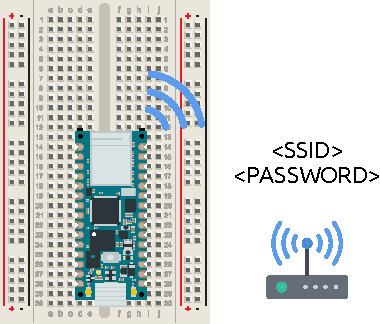
\includegraphics[width=0.65\textwidth]{images/microcontroller/exercises/exercise-4-solution.pdf}
        \caption{Solution for Exercise IV.}
    \end{figure}
\end{frame}

\begin{frame}{Solution: Exercise IV}
    \begin{listing}[H]
        \only<1>{\inputsource[fontsize=\fontsize{8}{8}, firstline=1, lastline=10]{c}{arduino/https-request.c}[hidealllines=true, tikzsetting={draw=black, line width=0.35pt}, leftline=true, rightline=true, topline=true]}
        \only<2>{\inputsource[fontsize=\fontsize{8}{8}, firstline=1, lastline=10, highlightlines=10]{c}{arduino/https-request.c}[hidealllines=true, tikzsetting={draw=black, line width=0.35pt}, leftline=true, rightline=true, topline=true]}
        \vspace{-1.25em}
        \inputsource[fontsize=\fontsize{8}{8}, firstline=38, lastline=38]{c}{arduino/https-request.c}[hidealllines=true, tikzsetting={draw=black, line width=0.35pt}, leftline=true, rightline=true]
        \vspace{-1.25em}
        \inputsource[fontsize=\fontsize{8}{8}, firstline=40, lastline=40]{c}{arduino/https-request.c}[hidealllines=true, tikzsetting={draw=black, line width=0.35pt}, leftline=true, rightline=true]
        \vspace{-1.25em}
        \inputsource[fontsize=\fontsize{8}{8}, firstline=55, lastline=55]{c}{arduino/https-request.c}[hidealllines=true, tikzsetting={draw=black, line width=0.35pt}, leftline=true, rightline=true]
        \vspace{-1.25em}
        \inputsource[fontsize=\fontsize{8}{8}, firstline=57, lastline=57]{c}{arduino/https-request.c}[hidealllines=true, tikzsetting={draw=black, line width=0.35pt}, leftline=true, rightline=true]
        \vspace{-1.25em}
        \inputsource[fontsize=\fontsize{8}{8}, firstline=67, lastline=67]{c}{arduino/https-request.c}[hidealllines=true, tikzsetting={draw=black, line width=0.35pt}, leftline=true, rightline=true, bottomline=true]
        \caption{Solution for Exercise IV.}
        \label{lst:arduino:exercise:4:solution:overview}
    \end{listing}
\end{frame}

\begin{frame}{Solution: Exercise IV}
    \begin{listing}[H]
        \only<1>{\inputsource[fontsize=\fontsize{8}{8}, firstline=10, lastline=38]{c}{arduino/https-request.c}}
        \only<2>{\inputsource[fontsize=\fontsize{8}{8}, firstline=10, lastline=38, highlightlines=26]{c}{arduino/https-request.c}}
        \caption{Solution for Exercise IV (\mintinline{c}{setup()}).}
        \label{lst:arduino:exercise:4:solution:part:1}
    \end{listing}
\end{frame}

\begin{frame}{Solution: Exercise IV}
    \begin{listing}[H]
        \inputsource[firstline=57, lastline=67]{c}{arduino/https-request.c}
        \caption{Solution for Exercise IV (\mintinline{c}{printWiFiStatus()}).}
        \label{lst:arduino:exercise:4:solution:part:2}
    \end{listing}
\end{frame}

\begin{frame}{Solution: Exercise IV}
    \begin{listing}[H]
        \inputsource[firstline=40, lastline=55]{c}{arduino/https-request.c}
        \caption{Solution for Exercise IV (\mintinline{c}{loop()}).}
        \label{lst:arduino:exercise:4:solution:part:3}
    \end{listing}
\end{frame}

\begin{frame}{Solution: Exercise IV}
    \begin{listing}[H]
        \inputsource[lastline=5]{sh}{arduino/https-request.example}
        \caption{Example output of solution for Exercise IV.}
        \label{lst:arduino:exercise:4:solution:output:part:1}
    \end{listing}
\end{frame}

\begin{frame}{Solution: Exercise IV}
    \begin{listing}[H]
        \inputsource[fontsize=\fontsize{8}{8}, firstline=7, lastline=26]{sh}{arduino/https-request.example}[hidealllines=true, tikzsetting={draw=black, line width=0.35pt}, leftline=true, rightline=true, topline=true]
        \vspace{-1.25em}
        \inputsource[fontsize=\fontsize{8}{8}, firstline=58, lastline=70]{sh}{arduino/https-request.example}[hidealllines=true, tikzsetting={draw=black, line width=0.35pt}, leftline=true, rightline=true, bottomline=true]
        \caption{Example output of solution for Exercise IV.}
        \label{lst:arduino:exercise:4:solution:output:part:2}
    \end{listing}
\end{frame}